\documentclass[a4paper,11pt]{scrartcl} 
%\usepackage[warn]{mathtext}
\usepackage[T2A]{fontenc}
%\usepackage[koi8-r]{inputenc}
\usepackage[utf8]{inputenc}
\usepackage[english,russian]{babel}
\usepackage{indentfirst}%first paragraph indent
\usepackage{cmap}
\usepackage[unicode=true]{hyperref}
\usepackage{graphicx}
\usepackage{amssymb}
\usepackage{amsmath}
\usepackage{srcltx}
\usepackage{textcomp}
\usepackage{floatflt}
\usepackage{wrapfig}
\usepackage{afterpage}
\usepackage{ccaption}
\captiondelim{. }
\usepackage{xspace}

\usepackage{wasysym}
\usepackage[noae]{Sweave}
\usepackage{underscore}
\deffootnote[2.5em]{1.5em}{1em}{\textsuperscript{\thefootnotemark}}
\setkomafont{sectioning}{\bfseries}
\setkomafont{descriptionlabel}{\bfseries}


%backslash
\newcommand{\bs}{\symbol{'134}}
%degree
\newcommand{\grad}{\ensuremath{{}^{\circ}}\xspace}
%R-акроним
\newcommand{\R}{{\sffamily\bfseries R}\xspace}

\title{Graphs  in  \R \\ and how it ?}
\author{ Stefanovskiy D }

\begin{document}
\maketitle

%\tableofcontents


\section{Creating  graphs}
\label{sec:smallgraph}


\begin{Schunk}
\begin{Sinput}
> library("igraph")
\end{Sinput}
\begin{Soutput}
[1] "igraph"    "stats"     "graphics"  "grDevices" "utils"     "datasets" 
[7] "methods"   "base"     
\end{Soutput}
\begin{Sinput}
> ver <- data.frame(name = c("Store1", "Store2", "Shop1", "Shop2", 
+     "Source", "Dest"), opport_requir = c(150, 50, 160, 40, 0, 
+     0))
\end{Sinput}
\begin{Soutput}
    name opport_requir
1 Store1           150
2 Store2            50
3  Shop1           160
4  Shop2            40
5 Source             0
6   Dest             0
\end{Soutput}
\begin{Sinput}
> relations <- data.frame(from = c("Source", "Source", "Shop1", 
+     "Shop2", "Store1", "Store2", "Store1", "Store2"), to = c("Store1", 
+     "Store2", "Dest", "Dest", "Shop1", "Shop2", "Shop2", "Shop1"), 
+     capacity = c(150, 50, 160, 40, 200, 200, 200, 200), price = c(150, 
+         50, 160, 40, 200, 200, 200, 200))
\end{Sinput}
\begin{Soutput}
    from     to capacity price
1 Source Store1      150   150
2 Source Store2       50    50
3  Shop1   Dest      160   160
4  Shop2   Dest       40    40
5 Store1  Shop1      200   200
6 Store2  Shop2      200   200
7 Store1  Shop2      200   200
8 Store2  Shop1      200   200
\end{Soutput}
\begin{Sinput}
> g <- graph.data.frame(relations, directed = TRUE, vertices = ver)
\end{Sinput}
\begin{Soutput}
Vertices: 6 
Edges: 8 
Directed: TRUE 
Edges:
                        
[0] 'Source' -> 'Store1'
[1] 'Source' -> 'Store2'
[2] 'Shop1'  -> 'Dest'  
[3] 'Shop2'  -> 'Dest'  
[4] 'Store1' -> 'Shop1' 
[5] 'Store2' -> 'Shop2' 
[6] 'Store1' -> 'Shop2' 
[7] 'Store2' -> 'Shop1' 
\end{Soutput}
\begin{Sinput}
> print(g, e = TRUE, v = TRUE)
\end{Sinput}
\begin{Soutput}
Vertices: 6 
Edges: 8 
Directed: TRUE 
Vertex attributes:
      name opport_requir
[0] Store1           150
[1] Store2            50
[2]  Shop1           160
[3]  Shop2            40
[4] Source             0
[5]   Dest             0
Edges and their attributes:
                         capacity price
[0] 'Source' -> 'Store1'      150   150
[1] 'Source' -> 'Store2'       50    50
[2] 'Shop1'  -> 'Dest'        160   160
[3] 'Shop2'  -> 'Dest'         40    40
[4] 'Store1' -> 'Shop1'       200   200
[5] 'Store2' -> 'Shop2'       200   200
[6] 'Store1' -> 'Shop2'       200   200
[7] 'Store2' -> 'Shop1'       200   200
Vertices: 6 
Edges: 8 
Directed: TRUE 
Edges:
                        
[0] 'Source' -> 'Store1'
[1] 'Source' -> 'Store2'
[2] 'Shop1'  -> 'Dest'  
[3] 'Shop2'  -> 'Dest'  
[4] 'Store1' -> 'Shop1' 
[5] 'Store2' -> 'Shop2' 
[6] 'Store1' -> 'Shop2' 
[7] 'Store2' -> 'Shop1' 
\end{Soutput}
\begin{Sinput}
> plot(g, vertex.shape = "crectangle", vertex.label = ver$name, 
+     edge.label = relations$capacity, layout = layout.graphopt)
\end{Sinput}
\begin{Soutput}
NULL
\end{Soutput}
\begin{Sinput}
> s = graph.maxflow(g, "Source", "Dest", capacity = relations$capacity)
\end{Sinput}
\begin{Soutput}
[1] 200
\end{Soutput}
\begin{Sinput}
> cat("maxflow =", s, "\n")
\end{Sinput}
\begin{Soutput}
maxflow = 200 
NULL
\end{Soutput}
\begin{Sinput}
> relations$capacity[5] = 110
\end{Sinput}
\begin{Soutput}
[1] 110
\end{Soutput}
\begin{Sinput}
> s = graph.maxflow(g, "Source", "Dest", capacity = relations$capacity)
\end{Sinput}
\begin{Soutput}
[1] 200
\end{Soutput}
\begin{Sinput}
> cat("maxflow =", s)
\end{Sinput}
\begin{Soutput}
maxflow = 200NULL
\end{Soutput}
\end{Schunk}
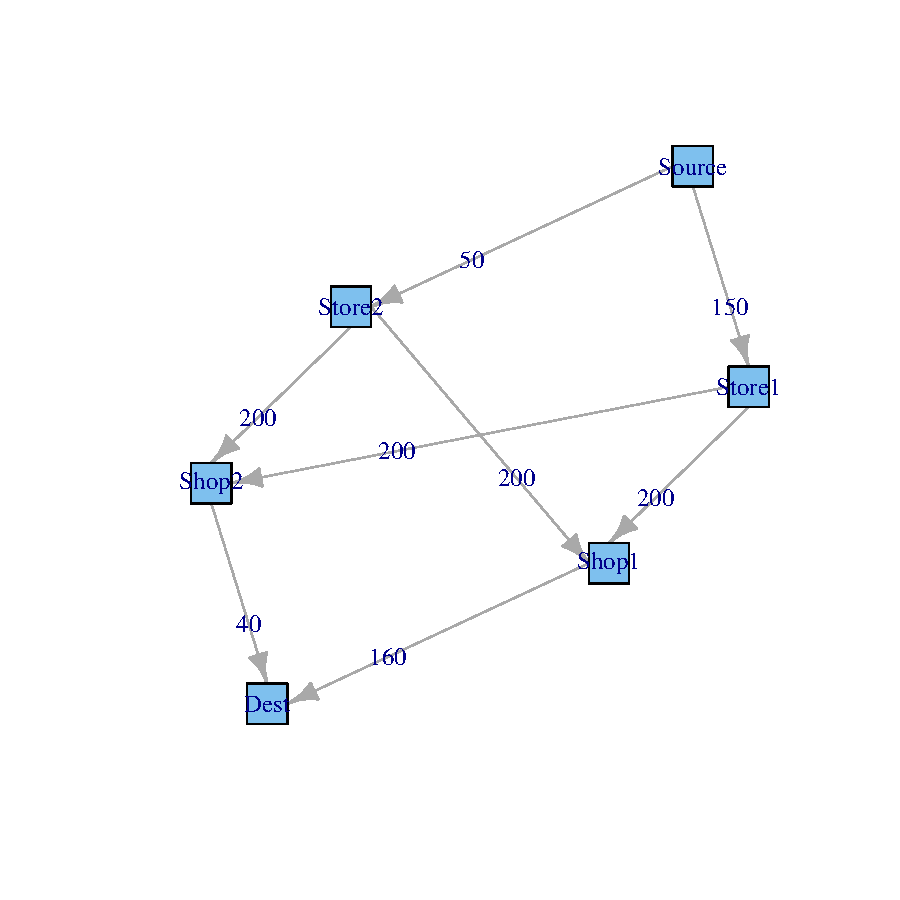
\includegraphics{graphs-001}

\end{document}
